

\tikzset{every picture/.style={line width=0.75pt}} %set default line width to 0.75pt        

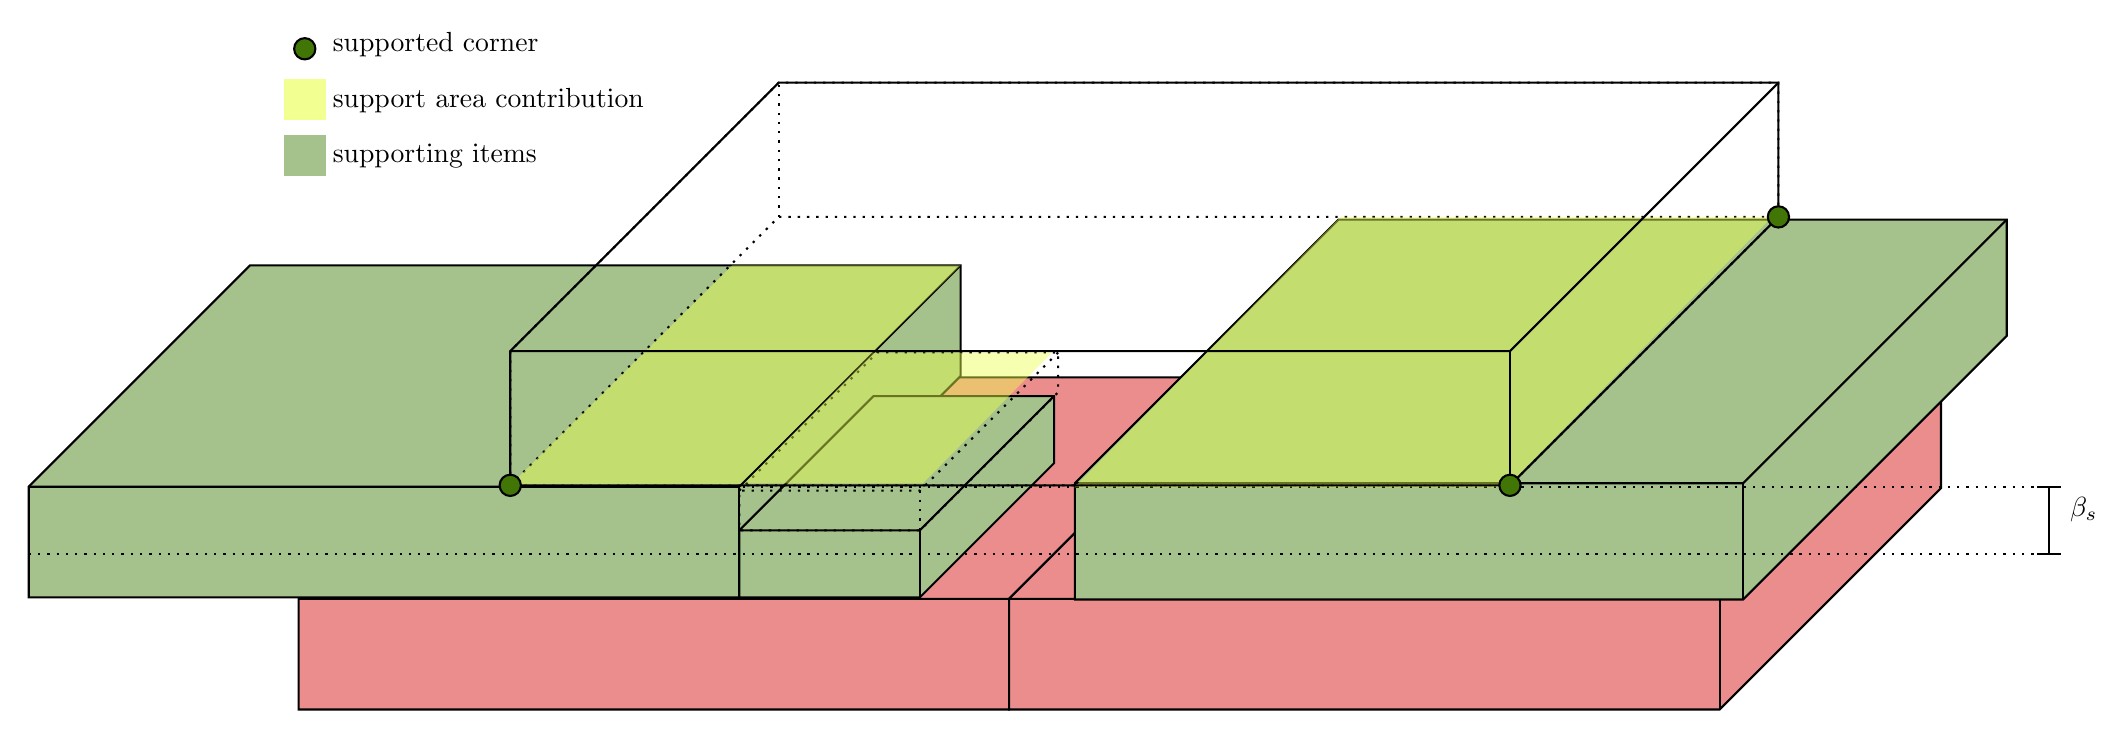
\begin{tikzpicture}[x=0.75pt,y=0.75pt,yscale=-1,xscale=1]
%uncomment if require: \path (0,479); %set diagram left start at 0, and has height of 479

%Shape: Cube [id:dp9411979483763162] 
\draw  [fill={rgb, 255:red, 236; green, 141; blue, 141 }  ,fill opacity=1 ] (194,306.67) -- (300.67,200) -- (643,200) -- (643,253.33) -- (536.33,360) -- (194,360) -- cycle ; \draw   (643,200) -- (536.33,306.67) -- (194,306.67) ; \draw   (536.33,306.67) -- (536.33,360) ;
%Shape: Cube [id:dp993645103603593] 
\draw  [fill={rgb, 255:red, 236; green, 141; blue, 141 }  ,fill opacity=1 ] (536.33,306.67) -- (643,200) -- (985.33,200) -- (985.33,253.33) -- (878.67,360) -- (536.33,360) -- cycle ; \draw   (985.33,200) -- (878.67,306.67) -- (536.33,306.67) ; \draw   (878.67,306.67) -- (878.67,360) ;
%Shape: Cube [id:dp23986673546182513] 
\draw  [fill={rgb, 255:red, 165; green, 194; blue, 140 }  ,fill opacity=1 ] (64,252.67) -- (170.67,146) -- (513,146) -- (513,199.33) -- (406.33,306) -- (64,306) -- cycle ; \draw   (513,146) -- (406.33,252.67) -- (64,252.67) ; \draw   (406.33,252.67) -- (406.33,306) ;
%Shape: Cube [id:dp5474008601617114] 
\draw  [fill={rgb, 255:red, 165; green, 194; blue, 140 }  ,fill opacity=1 ] (406.33,273.67) -- (471,209) -- (558,209) -- (558,241.33) -- (493.33,306) -- (406.33,306) -- cycle ; \draw   (558,209) -- (493.33,273.67) -- (406.33,273.67) ; \draw   (493.33,273.67) -- (493.33,306) ;
%Shape: Cube [id:dp7313777533771082] 
\draw  [fill={rgb, 255:red, 165; green, 194; blue, 140 }  ,fill opacity=1 ] (568,251) -- (695,124) -- (1017,124) -- (1017,180) -- (890,307) -- (568,307) -- cycle ; \draw   (1017,124) -- (890,251) -- (568,251) ; \draw   (890,251) -- (890,307) ;
%Shape: Cube [id:dp9978562503762016] 
\draw  [dash pattern={on 0.84pt off 2.51pt}] (907,122.67) -- (777.67,252) -- (296,252) -- (296,187.33) -- (425.33,58) -- (907,58) -- cycle ; \draw  [dash pattern={on 0.84pt off 2.51pt}] (296,252) -- (425.33,122.67) -- (907,122.67) ; \draw  [dash pattern={on 0.84pt off 2.51pt}] (425.33,122.67) -- (425.33,58) ;
%Shape: Cube [id:dp48964002783685845] 
\draw  [color={rgb, 255:red, 0; green, 0; blue, 0 }  ,draw opacity=1 ][fill={rgb, 255:red, 255; green, 255; blue, 255 }  ,fill opacity=0 ][dash pattern={on 0.84pt off 2.51pt}] (406.33,254.53) -- (472.86,188) -- (560,188) -- (560,207.14) -- (493.47,273.67) -- (406.33,273.67) -- cycle ; \draw  [color={rgb, 255:red, 0; green, 0; blue, 0 }  ,draw opacity=1 ][dash pattern={on 0.84pt off 2.51pt}] (560,188) -- (493.47,254.53) -- (406.33,254.53) ; \draw  [color={rgb, 255:red, 0; green, 0; blue, 0 }  ,draw opacity=1 ][dash pattern={on 0.84pt off 2.51pt}] (493.47,254.53) -- (493.47,273.67) ;
%Straight Lines [id:da26590658600836115] 
\draw    (1037.33,252.67) -- (1037.33,285) ;
\draw [shift={(1037.33,285)}, rotate = 270] [color={rgb, 255:red, 0; green, 0; blue, 0 }  ][line width=0.75]    (0,5.59) -- (0,-5.59)   ;
\draw [shift={(1037.33,252.67)}, rotate = 270] [color={rgb, 255:red, 0; green, 0; blue, 0 }  ][line width=0.75]    (0,5.59) -- (0,-5.59)   ;
%Straight Lines [id:da8302030012021052] 
\draw  [dash pattern={on 0.84pt off 2.51pt}]  (64,285) -- (1044,285) ;
%Straight Lines [id:da5354149137938202] 
\draw  [dash pattern={on 0.84pt off 2.51pt}]  (64,252.67) -- (1044,252.67) ;
%Shape: Parallelogram [id:dp4597753988697182] 
\draw  [color={rgb, 255:red, 0; green, 0; blue, 0 }  ,draw opacity=0 ][fill={rgb, 255:red, 234; green, 255; blue, 77 }  ,fill opacity=0.45 ] (403,146) -- (513,146) -- (406,252) -- (296,252) -- cycle ;
%Shape: Parallelogram [id:dp9407100355043312] 
\draw  [color={rgb, 255:red, 0; green, 0; blue, 0 }  ,draw opacity=0 ][fill={rgb, 255:red, 234; green, 255; blue, 77 }  ,fill opacity=0.45 ] (471,188) -- (557,188) -- (494.86,251) -- (408.86,251) -- cycle ;
%Shape: Parallelogram [id:dp5499917231467685] 
\draw  [color={rgb, 255:red, 0; green, 0; blue, 0 }  ,draw opacity=0 ][fill={rgb, 255:red, 234; green, 255; blue, 77 }  ,fill opacity=0.45 ] (696,122.67) -- (904,122.67) -- (775.67,253) -- (567.67,253) -- cycle ;
%Shape: Cube [id:dp21506487392572304] 
\draw   (296,187.33) -- (425.33,58) -- (907,58) -- (907,122.67) -- (777.67,252) -- (296,252) -- cycle ; \draw   (907,58) -- (777.67,187.33) -- (296,187.33) ; \draw   (777.67,187.33) -- (777.67,252) ;
%Shape: Rectangle [id:dp8515603217170198] 
\draw  [color={rgb, 255:red, 0; green, 0; blue, 0 }  ,draw opacity=0 ][fill={rgb, 255:red, 234; green, 255; blue, 77 }  ,fill opacity=0.62 ] (187,56) -- (207,56) -- (207,76) -- (187,76) -- cycle ;
%Shape: Rectangle [id:dp8969674268045522] 
\draw  [color={rgb, 255:red, 0; green, 0; blue, 0 }  ,draw opacity=0 ][fill={rgb, 255:red, 165; green, 194; blue, 140 }  ,fill opacity=1 ] (187,83) -- (207,83) -- (207,103) -- (187,103) -- cycle ;
%Shape: Circle [id:dp08410160878408413] 
\draw  [fill={rgb, 255:red, 65; green, 117; blue, 5 }  ,fill opacity=1 ] (290.88,252) .. controls (290.88,249.17) and (293.17,246.88) .. (296,246.88) .. controls (298.83,246.88) and (301.13,249.17) .. (301.13,252) .. controls (301.13,254.83) and (298.83,257.13) .. (296,257.13) .. controls (293.17,257.13) and (290.88,254.83) .. (290.88,252) -- cycle ;
%Shape: Circle [id:dp20799682119759832] 
\draw  [fill={rgb, 255:red, 65; green, 117; blue, 5 }  ,fill opacity=1 ] (772.54,252) .. controls (772.54,249.17) and (774.84,246.88) .. (777.67,246.88) .. controls (780.5,246.88) and (782.79,249.17) .. (782.79,252) .. controls (782.79,254.83) and (780.5,257.13) .. (777.67,257.13) .. controls (774.84,257.13) and (772.54,254.83) .. (772.54,252) -- cycle ;
%Shape: Circle [id:dp9242580914559287] 
\draw  [fill={rgb, 255:red, 65; green, 117; blue, 5 }  ,fill opacity=1 ] (901.88,122.67) .. controls (901.88,119.84) and (904.17,117.54) .. (907,117.54) .. controls (909.83,117.54) and (912.13,119.84) .. (912.13,122.67) .. controls (912.13,125.5) and (909.83,127.79) .. (907,127.79) .. controls (904.17,127.79) and (901.88,125.5) .. (901.88,122.67) -- cycle ;
%Shape: Circle [id:dp40386474009325335] 
\draw  [fill={rgb, 255:red, 65; green, 117; blue, 5 }  ,fill opacity=1 ] (191.88,41.67) .. controls (191.88,38.84) and (194.17,36.54) .. (197,36.54) .. controls (199.83,36.54) and (202.13,38.84) .. (202.13,41.67) .. controls (202.13,44.5) and (199.83,46.79) .. (197,46.79) .. controls (194.17,46.79) and (191.88,44.5) .. (191.88,41.67) -- cycle ;

% Text Node
\draw (1046,256.07) node [anchor=north west][inner sep=0.75pt]    {$\beta_{s}$};
% Text Node
\draw (209,59) node [anchor=north west][inner sep=0.75pt]   [align=left] {support area contribution};
% Text Node
\draw (209,86) node [anchor=north west][inner sep=0.75pt]   [align=left] {supporting items};
% Text Node
\draw (209,32) node [anchor=north west][inner sep=0.75pt]   [align=left] {supported corner};


\end{tikzpicture}
